\documentclass[book.tex]{subfiles}
\begin{document}
\section{Programming}
\label{section:programming}



Development was done with Borland C++ 3.1 (but the language used was C). John Carmack took care of the runtime code. John Romero programmed many of the tools (TED5 map editor, IGRAB asset packer, MUSE sound packer). Jason Blochowiak wrote important subsystems of the game (Input manager, Sound manager, User manager).\\
\par
Borland's solution was an all-in-one package. The IDE, \cw{BC.EXE}, despite some instabilities allowed crude multi-windows code editing with pleasant syntax highlights. The compiler and linker were also part of the package under \cw{BCC.EXE} and \cw{TLINK.EXE}\footnote{Source: Borland C++ 3.1 User Guide.}. There was no need to enter command-line mode however. The IDE allowed to create a project, build, run and debug. The software came with two thick manuals, explaining everything regarding the IDE and programming in C++.\\

\par
\begin{figure}[H]
\centering
\begin{minipage}{.5\textwidth}
  \centering
  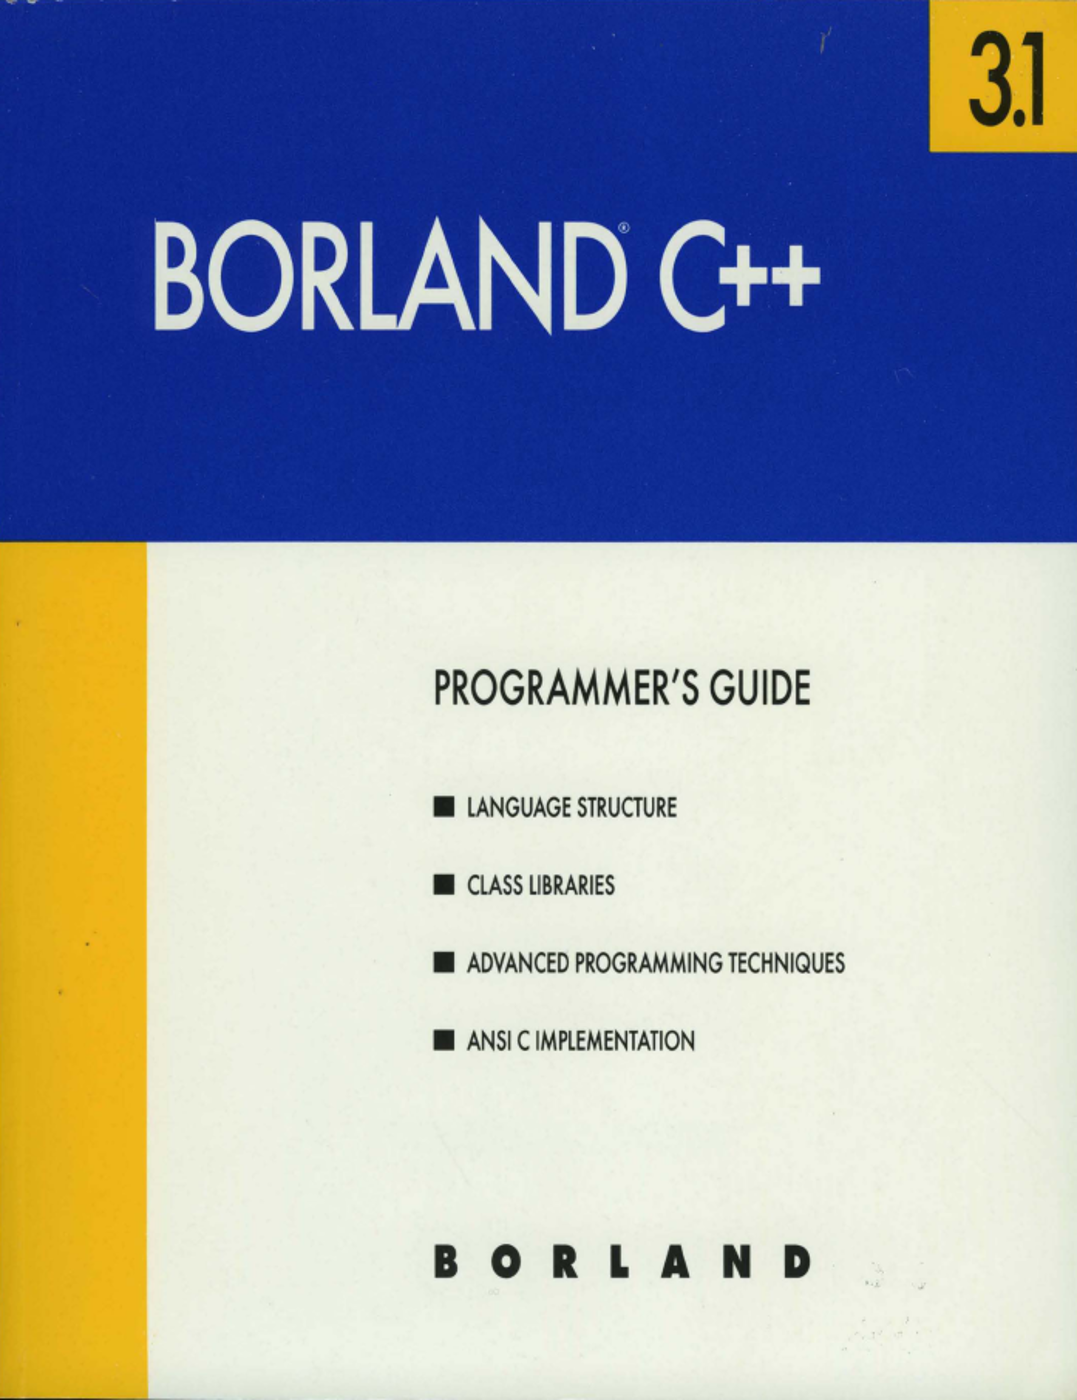
\includegraphics[width=.5\linewidth]{screenshots_300dpi/borland_programmer_guide.png}
\end{minipage}%
\begin{minipage}{.5\textwidth}
  \centering
  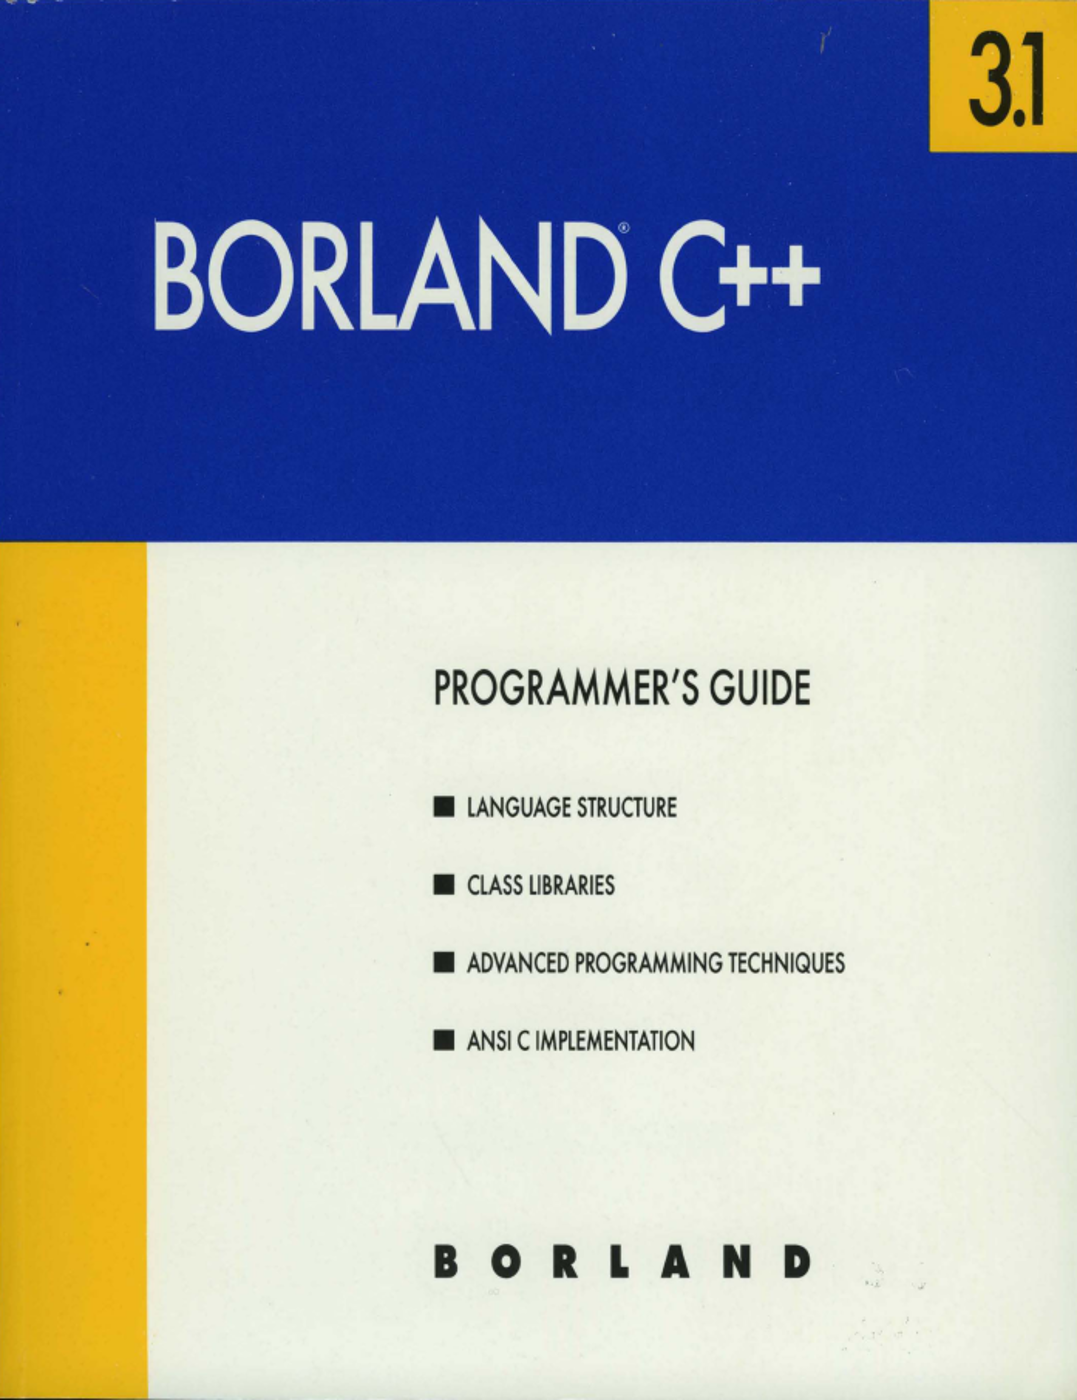
\includegraphics[width=.5\linewidth]{screenshots_300dpi/borland_programmer_guide.png}
\end{minipage}
\caption{Borland C++ 3.1 User guide (238 pages) and Programmer guide (483 pages).}
\end{figure}


\par
\begin{figure}[H]
\centering
  \fullimage{borland_memory_model.png}
\end{figure}

\par
\begin{figure}[H]
\centering
  \fullimage{borland_compile.png}
  \caption{Selecting memory model and compiling Keen Dreams with Borland C++ 3.1}
\end{figure}




\section{Graphic Assets}
\label{section:graphic_assets}

All graphic assets were produced by Adrian Carmack. All of the work was done with Deluxe Paint (by Brent Iverson, Electronic Arts) and saved in ILBM\footnote{InterLeaved BitMap.} files (Deluxe Paint proprietary format). All assets were hand drawn with a mouse.

\begin{figure}[H]
  \centering
 \fullimage{deluxe_paint.png}
 \caption{Deluxe Paint was used to draw all assets in the game.}
\end{figure}

\subsection{Tile introduction}
Before diving into the details of game assets, let's first explore the basic principles behind platform games. Each level, or map, in a platform game is composed of "tiles". In Commander Keen, there are both background and foreground tiles. A background tile, or just "tile", is an image that measures 16x16 pixels. Each tile occupies 128 bytes (2 x 16 x 4 planes) of storage space in the graphics assets file.\\

\par
Individual tile images are stored in a planar format, with blue, green, red and intensity bits separated. This arrangement, called "graphic planar", stores complete planes sequentially, with each plane containing data for the entire tile.\\

\par
\begin{figure}[H]
\centering
 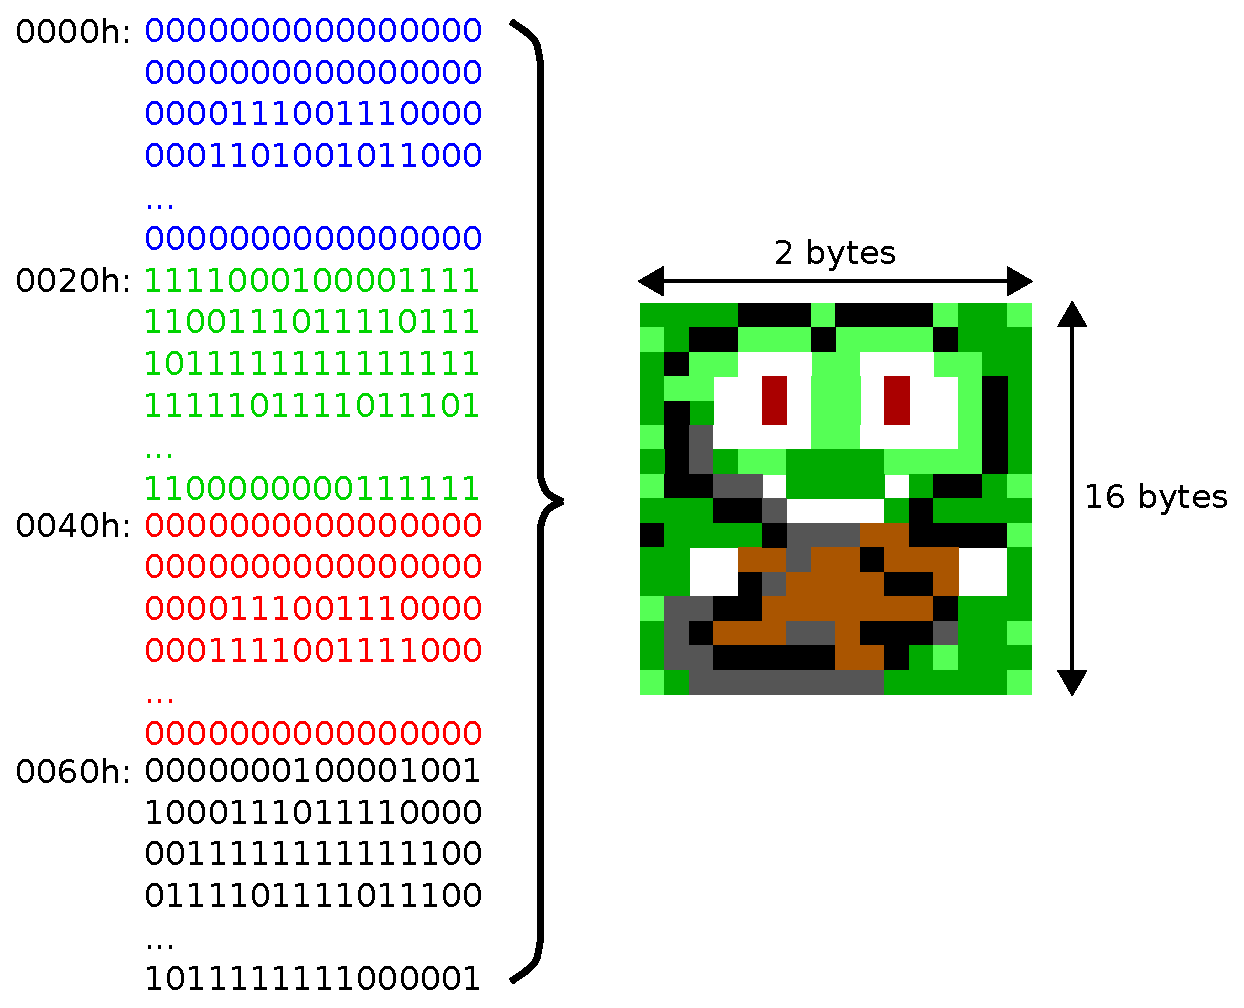
\includegraphics[width=.8\textwidth]{imgs/drawings/Tile_RGBI.eps}
 \caption{Graphic Planar data storage.}
 \label{graphic_planar}
\end{figure}

\par
Foreground tiles, or "masked tiles", are similar to normal tiles but contain five planes instead of four. The extra plane stores the mask, and the order of planes is mask, blue, green, red, intensity. Consequently, a single masked tile requires 160 bytes (128 + 32) of storage. A mask bit of '0' means the background tile color is erased and replaced by the foreground tile color, while a mask bit of '1' blends the background color with the foreground color. If the foreground color is '0', the background color remains visible. \\

\par
By combining tiles on the screen, a map is created. These maps define the entire game world in terms of background and foreground tiles. Maps also contain a list of all actors and their starting positions within the world. Essentially, everything the player encounters while progressing through the levels is specified in a map.

\subsection{Assets Workflow}
After the graphic assets were generated, a tool (IGRAB) packed all ILBM files into a compressed data asset file (\cw{EGA}-file) and generated a \cw{HEAD} table, \cw{DICT} file (\cw{KDR}-files\footnote{both \cw{KDR}-files are located in the \cw{static} folder of the source code.}), and a C header file containing asset IDs. The engine references an asset directly using these IDs.\\


\begin{figure}[H]
\centering
 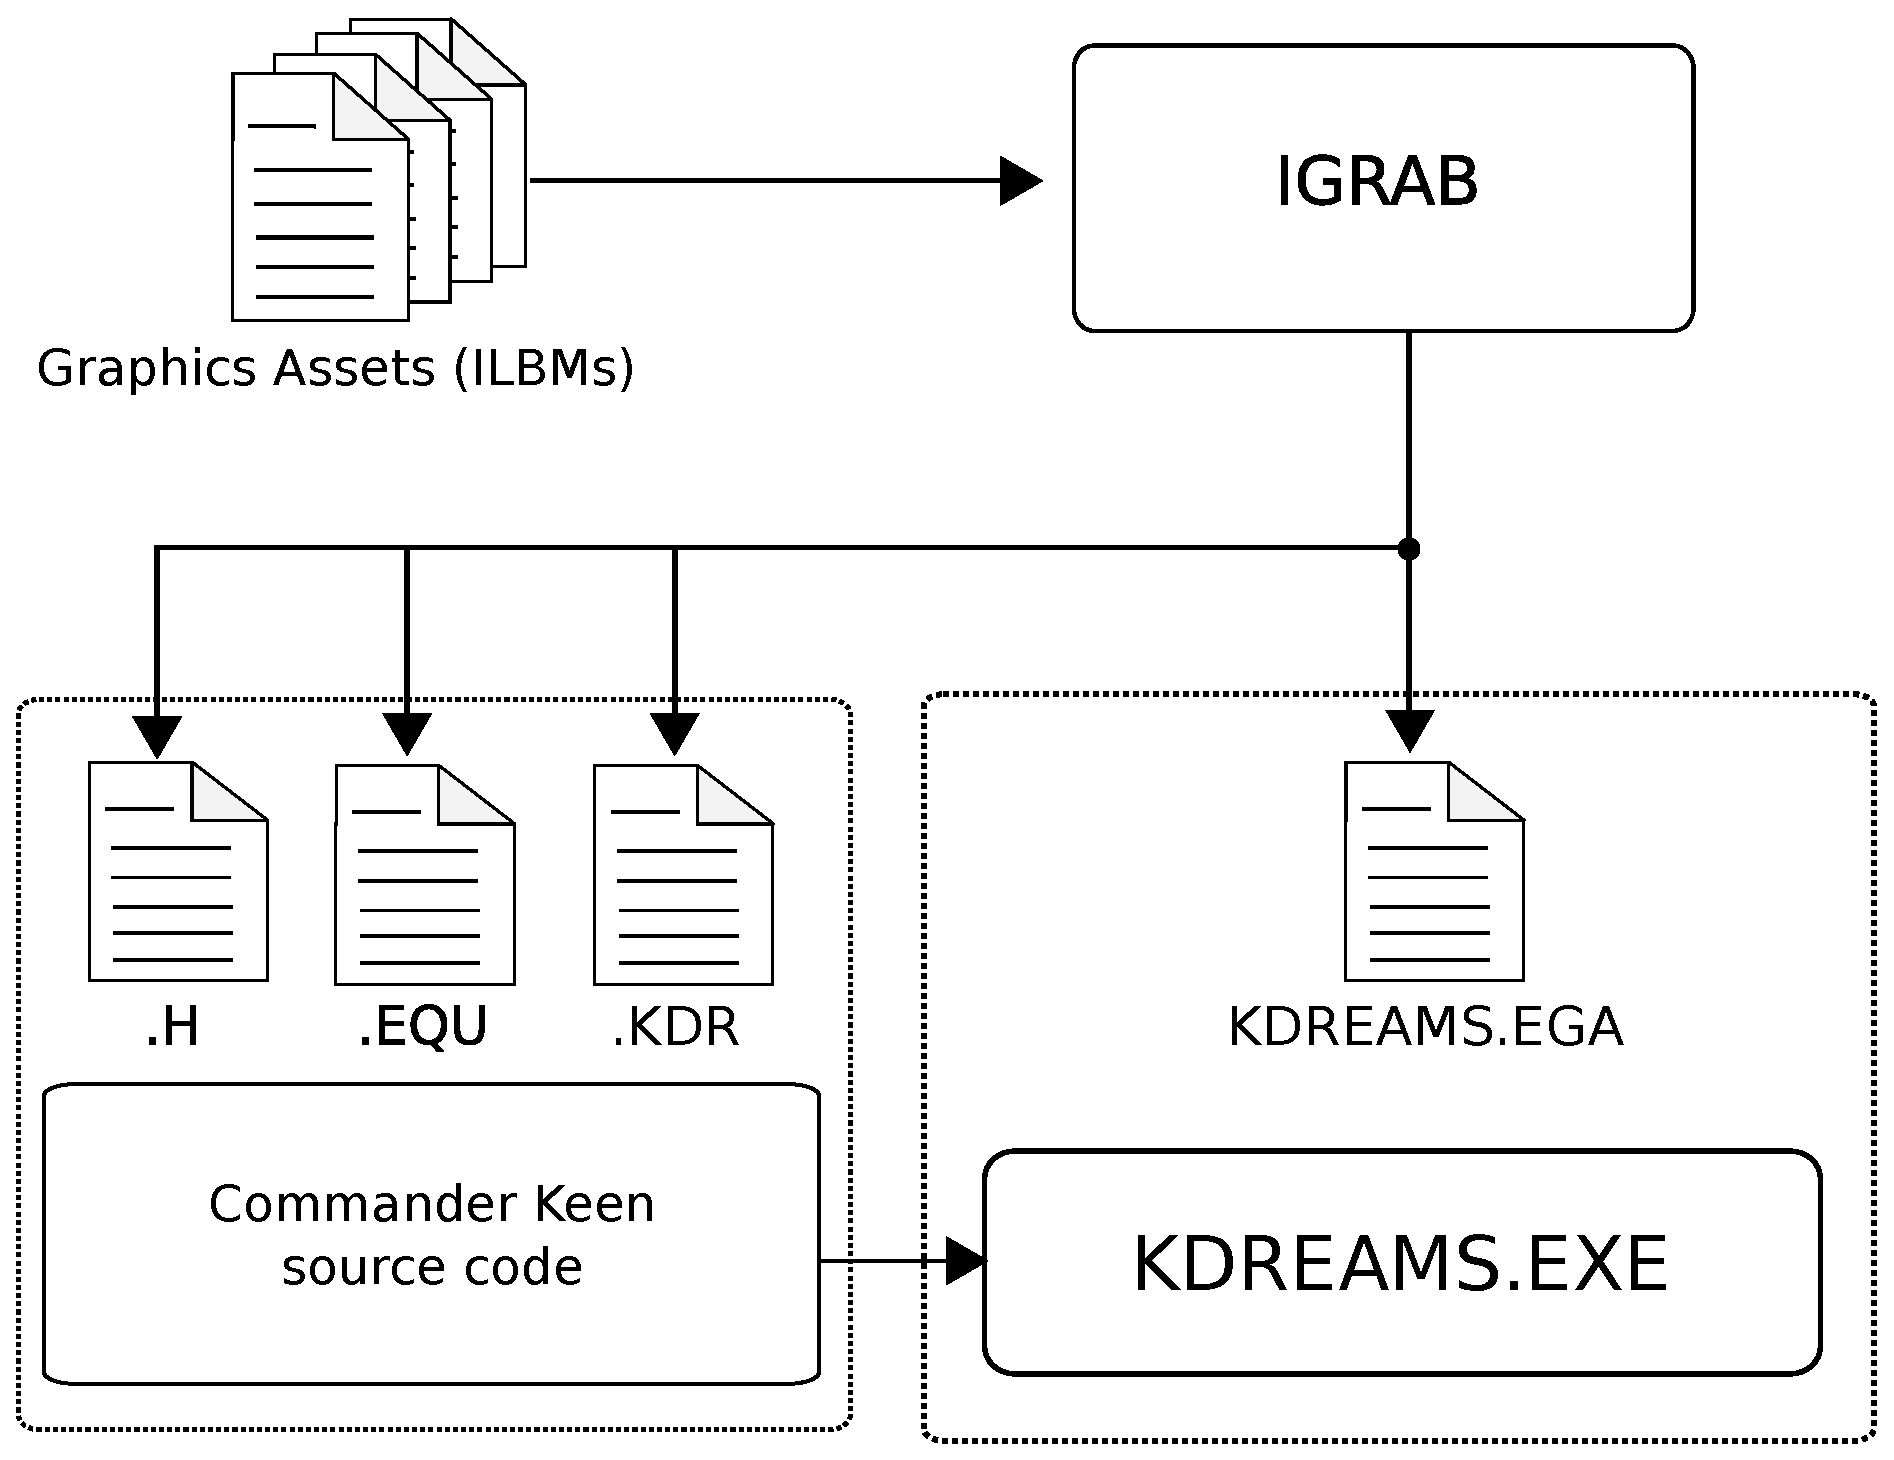
\includegraphics[width=.9\textwidth]{imgs/drawings/drawing_plain.eps}
 \caption{Asset creation pipeline for graphics items}
 \label{asset-creation-pipeline}
\end{figure}

\par
In the engine's code, asset usage is hardcoded via an enum. This enum serves as an offset into the \cw{HEAD} table, which then provides an offset within the data asset file. With this indirection layer, assets could be regenerated and reordered at will with no modification in the source code.\\

\trivia{The \cw{HEAD} and \cw{DICT} files in the source code must match the data asset file from the shareware version of \textit{Keen Dreams}. However, the latest release of the source code (v1.93) does not match with shareware version v1.13. To ensure that the \cw{HEAD}, \cw{DICT}, and data asset file are compatible, you will need to retrieve a specific git commit, which will be explained in the next chapter.}


\par
\begin{minipage}{\textwidth}
 \lstinputlisting[language=C]{code/assets_header.c}\par
 \end{minipage}
  

\subsection{Assets file structure}
\label{section:asset_file_structure}
Figure \ref{fig:asset-file} illustrates the structure of the \cw{KDREAMS.EGA} asset file. The first section contains data tables for pictures and sprites, followed by the font, and all sprite and tile graphs. 

\begin{figure}[H]
\centering
 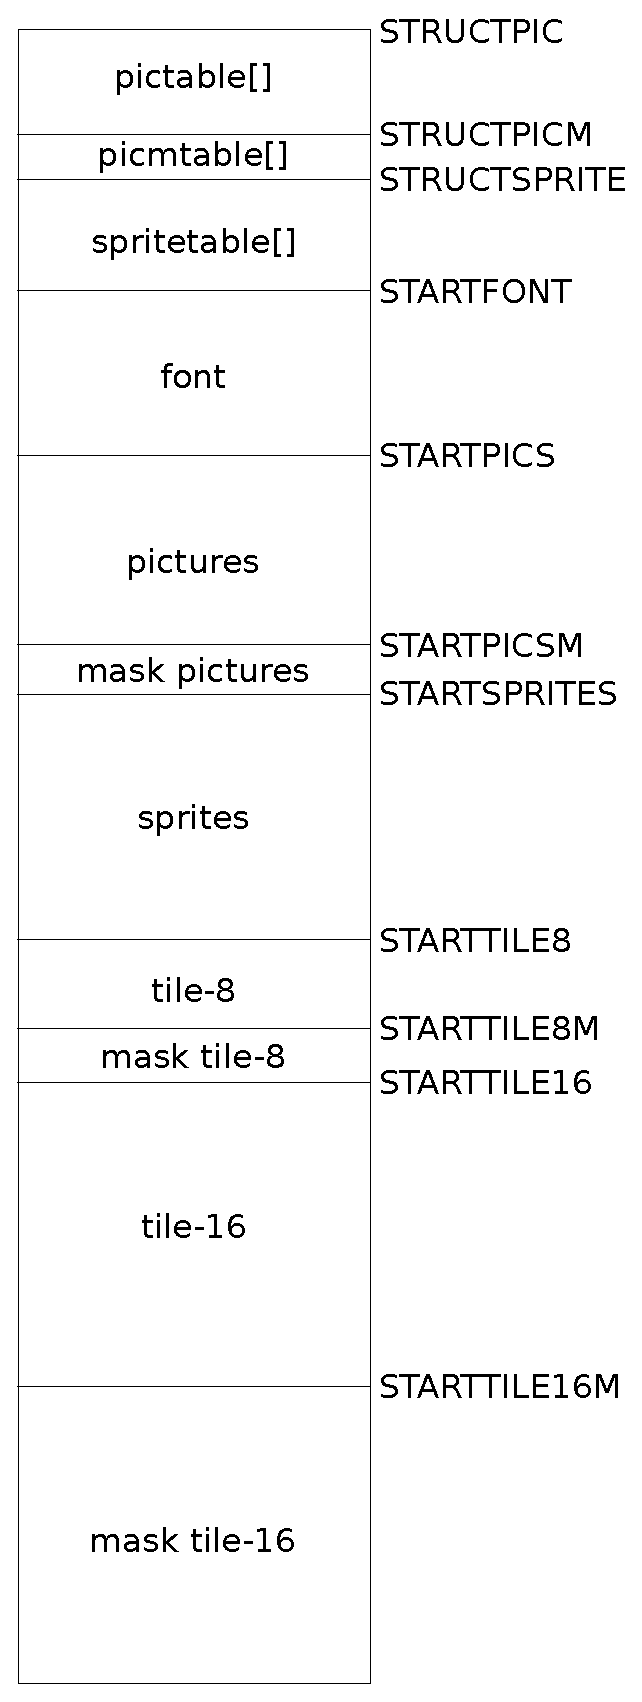
\includegraphics[width=.4\textwidth]{imgs/drawings/graphic_assets.eps}
 \caption{File structure of \cw{KDREAMS.EGA} archive file.}
 \label{fig:asset-file}
\end{figure}

\pagebreak
Both the \cw{pictable[]} and \cw{picmtable[]} contain the width and height for each (masked) picture in the asset file.\\
  \begin{table}[H]
  \begin{tabularx}{0.8\textwidth}[c]{XXX}
  \hline
  \textbf{picture index} & \textbf{width (bytes)} & \textbf{height (bytes)}   \\ \hline
  0             & 5          & 32    \\
  1             & 5          & 32    \\
  2             & 5          & 32    \\
  3             & 5          & 32    \\
  4             & 5          & 32    \\
  5             & 5          & 32    \\
  6             & 5          & 32    \\
  7             & 5          & 32    \\
  ...             & ...          & ...    \\
  64             & 5          & 24    \\
  \end{tabularx}
  %\caption{content of \cw{pictable[]} and \cw{picmtable[]}.}
  \end{table}

\par
The \cw{spritetable[]} includes not only width and height but also information on the sprite's center, hitbox, and number of bit shifts (explained in Section \ref{section:actors_and_sprites} on page \pageref{section:actors_and_sprites}). \\

\par
\begin{minipage}{\textwidth}
 \lstinputlisting[language=C]{code/sprite_structure.c}\par
 \end{minipage}\\


\par
All sprite placement occurs from the origin, which is offset by \cw{(orgx, orgy)} from the sprite's top-left corner. The parameters \cw{(xl, xh, yl, yh)} define the sprite's hitbox, used for collision detection. Sprites have an additional layer to indicate transparency, similar to masked tiles.\\

\par
\begin{figure}[H]
\centering
\begin{minipage}{.5\textwidth}
  \centering
  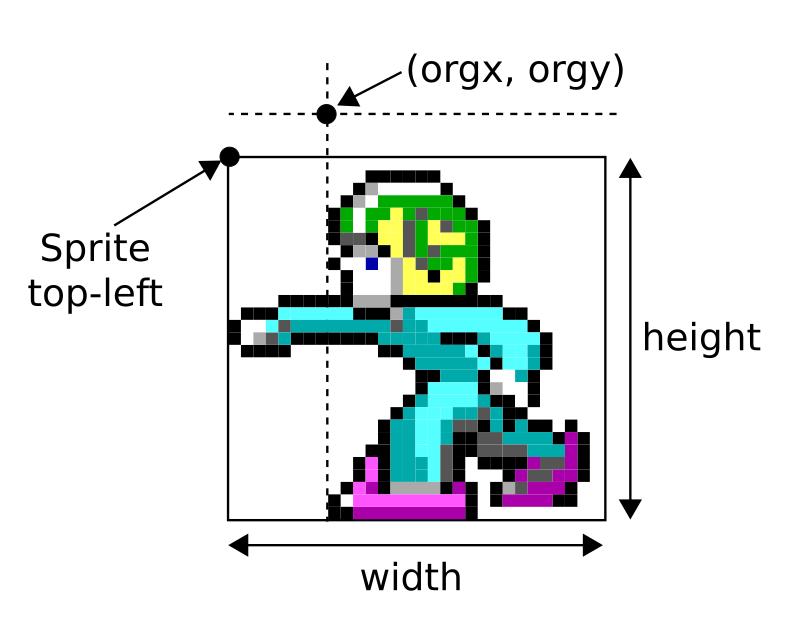
\includegraphics[width=1.0\linewidth]{imgs/drawings/sprite_origin.png}
\end{minipage}%
\begin{minipage}{.5\textwidth}
  \centering
  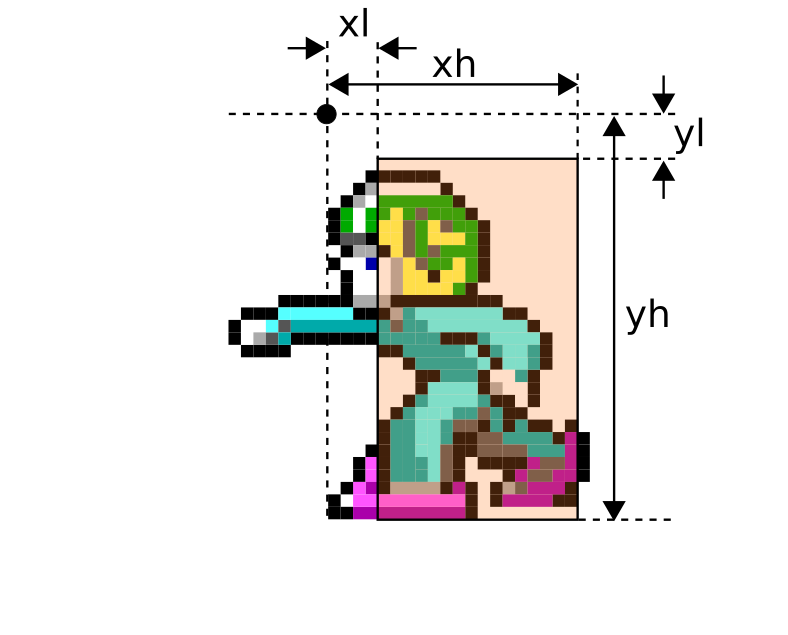
\includegraphics[width=1.0\linewidth]{imgs/drawings/sprite_hitbox.png}
\end{minipage}
\caption{Sprite dimensions, origin and hitbox.}
\label{fig:sprite_structure}
\end{figure}


\par
The font segment contains a table that stores the height and the width of the font, along with a reference to where the character data is located in the archive file.\\


\par
\begin{minipage}{\textwidth}
 \lstinputlisting[language=C]{code/font_structure.c}\par
 \end{minipage}


\par
\begin{figure}[H] 
  \centering 
  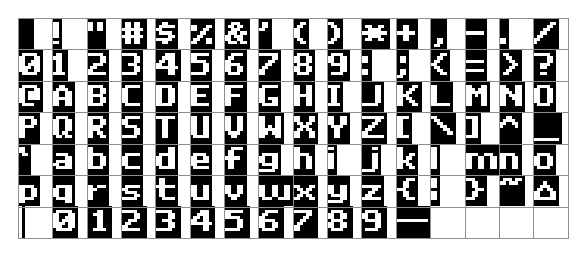
\includegraphics[width=1.0\textwidth]{imgs/drawings/font.eps}
  \caption{Font asset data.}
  \label{fig:font_assets}
\end{figure} 

\pagebreak
The remainder of the archive file holds all graphic assets, including pictures, sprites, and tiles. Each asset contains four planes, aligned with the EGA architecture. All masked tiles and sprites also include an additional mask plane.\\



\par 
\begin{figure}[H]
\centering
 \begin{table}[H]
  \begin{tabularx}{\textwidth}[c]{XXXXXX}
  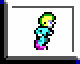
\includegraphics[width=0.15\textwidth]{screenshots_300dpi/game/picture01.jpg} &
  
\includegraphics[width=0.15\textwidth]{screenshots_300dpi/game/picture02.jpg} &
  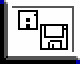
\includegraphics[width=0.15\textwidth]{screenshots_300dpi/game/picture03.jpg} &
  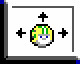
\includegraphics[width=0.15\textwidth]{screenshots_300dpi/game/picture04.jpg} &
  
\includegraphics[width=0.15\textwidth]{screenshots_300dpi/game/picture5.png} &
  
\includegraphics[width=0.15\textwidth]{screenshots_300dpi/game/picture6.png} \\
  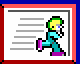
\includegraphics[width=0.15\textwidth]{screenshots_300dpi/game/picture7.png} &
  
\includegraphics[width=0.15\textwidth]{screenshots_300dpi/game/picture8.png} &
  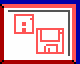
\includegraphics[width=0.15\textwidth]{screenshots_300dpi/game/picture9.png} &
  
\includegraphics[width=0.15\textwidth]{screenshots_300dpi/game/picture10.png} &
  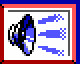
\includegraphics[width=0.15\textwidth]{screenshots_300dpi/game/picture11.jpg} &
  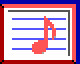
\includegraphics[width=0.15\textwidth]{screenshots_300dpi/game/picture12.jpg} \\
  
\includegraphics[width=0.15\textwidth]{screenshots_300dpi/game/picture13.jpg} &
  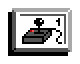
\includegraphics[width=0.15\textwidth]{screenshots_300dpi/game/picture14.jpg} &
  
\includegraphics[width=0.15\textwidth]{screenshots_300dpi/game/picture15.png} &
  
\includegraphics[width=0.15\textwidth]{screenshots_300dpi/game/picture16.jpg} &
  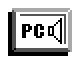
\includegraphics[width=0.15\textwidth]{screenshots_300dpi/game/picture17.jpg} &
  
\includegraphics[width=0.15\textwidth]{screenshots_300dpi/game/picture18.jpg} \\
  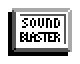
\includegraphics[width=0.15\textwidth]{screenshots_300dpi/game/picture19.jpg} &
  
\includegraphics[width=0.15\textwidth]{screenshots_300dpi/game/picture20.jpg} &
  
\includegraphics[width=0.15\textwidth]{screenshots_300dpi/game/picture21.jpg} &
  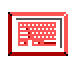
\includegraphics[width=0.15\textwidth]{screenshots_300dpi/game/picture22.jpg} &
  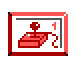
\includegraphics[width=0.15\textwidth]{screenshots_300dpi/game/picture23.jpg} &
  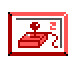
\includegraphics[width=0.15\textwidth]{screenshots_300dpi/game/picture24.jpg} \\
  
\includegraphics[width=0.15\textwidth]{screenshots_300dpi/game/picture25.jpg} &
  
\includegraphics[width=0.15\textwidth]{screenshots_300dpi/game/picture26.jpg} &
  
\includegraphics[width=0.15\textwidth]{screenshots_300dpi/game/picture27.jpg} &
  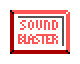
\includegraphics[width=0.15\textwidth]{screenshots_300dpi/game/picture28.jpg} &
  
\includegraphics[width=0.15\textwidth]{screenshots_300dpi/game/picture29.jpg} &
  
\includegraphics[width=0.15\textwidth]{screenshots_300dpi/game/picture30.jpg} \\
  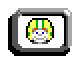
\includegraphics[width=0.15\textwidth]{screenshots_300dpi/game/picture31.jpg} &
  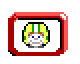
\includegraphics[width=0.15\textwidth]{screenshots_300dpi/game/picture32.jpg} &
  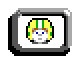
\includegraphics[width=0.15\textwidth]{screenshots_300dpi/game/picture33.jpg} &
  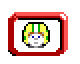
\includegraphics[width=0.15\textwidth]{screenshots_300dpi/game/picture34.jpg} &
  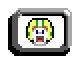
\includegraphics[width=0.15\textwidth]{screenshots_300dpi/game/picture35.jpg} &
  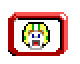
\includegraphics[width=0.15\textwidth]{screenshots_300dpi/game/picture36.jpg} \\
  
\includegraphics[width=0.15\textwidth]{screenshots_300dpi/game/picture37.jpg} &
  
\includegraphics[width=0.15\textwidth]{screenshots_300dpi/game/picture38.jpg} &
  
\includegraphics[width=0.15\textwidth]{screenshots_300dpi/game/picture39.jpg} &
  
\includegraphics[width=0.15\textwidth]{screenshots_300dpi/game/picture40.jpg} &
  
\includegraphics[width=0.15\textwidth]{screenshots_300dpi/game/picture41.jpg} &
  
\includegraphics[width=0.15\textwidth]{screenshots_300dpi/game/picture42.jpg} \\
  \end{tabularx}
  \end{table}
  \caption{Picture assets.}
  \label{fig:picture_assets}
 \end{figure} 
 

\begin{figure}[H]
\centering
 \begin{table}[H]
  \begin{tabularx}{\textwidth}[c]{|XXXXXX|}
  \hline
  \includegraphics[width=0.17\textwidth]{screenshots_300dpi/game/sprite1a.png} &
  \includegraphics[width=0.17\textwidth]{screenshots_300dpi/game/sprite1b.png} &
  \includegraphics[width=0.17\textwidth]{screenshots_300dpi/game/sprite1c.png} &
  \includegraphics[width=0.17\textwidth]{screenshots_300dpi/game/sprite1d.png} &
  \includegraphics[width=0.17\textwidth]{screenshots_300dpi/game/sprite1e.png} &
  \includegraphics[width=0.17\textwidth]{screenshots_300dpi/game/sprite1f.png} \\  
  \includegraphics[width=0.17\textwidth]{screenshots_300dpi/game/sprite1g.png} & 
  \includegraphics[width=0.17\textwidth]{screenshots_300dpi/game/sprite1h.png} &
  \includegraphics[width=0.17\textwidth]{screenshots_300dpi/game/sprite2a.png} &
  \includegraphics[width=0.17\textwidth]{screenshots_300dpi/game/sprite2b.png} &
  \includegraphics[width=0.17\textwidth]{screenshots_300dpi/game/sprite2c.png} &
  \includegraphics[width=0.17\textwidth]{screenshots_300dpi/game/sprite2d.png} \\  
  \includegraphics[width=0.17\textwidth]{screenshots_300dpi/game/sprite2e.png} &
  \includegraphics[width=0.17\textwidth]{screenshots_300dpi/game/sprite2f.png} &
  \includegraphics[width=0.17\textwidth]{screenshots_300dpi/game/sprite2g.png} & 
  \includegraphics[width=0.17\textwidth]{screenshots_300dpi/game/sprite2h.png} & & \\  
  \multicolumn{6}{|c|}{BROCCOLASH}  \\ \hline
  \multicolumn{6}{c}{}  \\ \hline    
  
  \includegraphics[width=0.17\textwidth]{screenshots_300dpi/game/sprite3e.png} &
  \includegraphics[width=0.17\textwidth]{screenshots_300dpi/game/sprite3f.png} &
  \includegraphics[width=0.17\textwidth]{screenshots_300dpi/game/sprite3g.png} & 
  \includegraphics[width=0.17\textwidth]{screenshots_300dpi/game/sprite3h.png} &   
  \includegraphics[width=0.17\textwidth]{screenshots_300dpi/game/sprite4a.png} &
  \includegraphics[width=0.17\textwidth]{screenshots_300dpi/game/sprite4b.png} \\    
  \includegraphics[width=0.17\textwidth]{screenshots_300dpi/game/sprite4c.png} &
  \includegraphics[width=0.17\textwidth]{screenshots_300dpi/game/sprite4d.png} &
  \includegraphics[width=0.17\textwidth]{screenshots_300dpi/game/sprite4e.png} & 
  \includegraphics[width=0.17\textwidth]{screenshots_300dpi/game/sprite4f.png} & & \\
  \multicolumn{6}{|c|}{CARROT}  \\ \hline
  \multicolumn{6}{c}{}   \\ \hline
  
  \includegraphics[width=0.17\textwidth]{screenshots_300dpi/game/sprite5a.png} &
  \includegraphics[width=0.17\textwidth]{screenshots_300dpi/game/sprite5b.png} &  
  \includegraphics[width=0.17\textwidth]{screenshots_300dpi/game/sprite5c.png} &
  \includegraphics[width=0.17\textwidth]{screenshots_300dpi/game/sprite5d.png} &  
  \includegraphics[width=0.17\textwidth]{screenshots_300dpi/game/sprite5e.png} &
  \includegraphics[width=0.17\textwidth]{screenshots_300dpi/game/sprite5f.png} \\
  \multicolumn{6}{|c|}{MELONLIPS}  \\ \hline
  \multicolumn{6}{c}{}    \\ \hline  
  
      
  \includegraphics[width=0.17\textwidth]{screenshots_300dpi/game/sprite3a.png} &
  \includegraphics[width=0.17\textwidth]{screenshots_300dpi/game/sprite3b.png} &  
  \includegraphics[width=0.17\textwidth]{screenshots_300dpi/game/sprite3c.png} &
  \includegraphics[width=0.17\textwidth]{screenshots_300dpi/game/sprite3d.png} & & \\  
  \multicolumn{6}{|c|}{TOMATOOTH}  \\ \hline
    
  \end{tabularx}
  \end{table}
  \caption{Sprite assets.}
  \label{fig:sprite_assets}
 \end{figure}


\pagebreak
\begin{figure}[H] 
  \centering 
  \includegraphics[width=0.99\textwidth, frame]{screenshots_300dpi/tile16_assets.png}
\end{figure}  

\begin{figure}[H] 
  \centering 
  \includegraphics[width=0.99\textwidth, frame]{screenshots_300dpi/tile16M_assets.png}
  \caption{Background (Tile-16) and foreground (masked Tile-16) assets.}
  \label{fig:tile16_assets}
\end{figure} 



\section{Maps}
Maps were created using an in-house editor called TED5, short for Tile EDitor. Over the years TED5 had improvements and the same tool is later used for creating maps for both side-scrolling games and top-down games like \textit{Wolfenstein 3D}.\\
\par
 TED5 is not stand-alone; in order to start, it needs an asset archive and the  associated header (as described in the graphic asset workflow Figure \ref{asset-creation-pipeline} on page \pageref{asset-creation-pipeline}). This way, tile IDs are directly encoded in the map.\\

 
 \fullimage{TedSplashscreen.png}
 \par
 \trivia{The suffix, "vD.IP", was put in by the Rise of the Triad team in 1994. It stood for "Developers of Incredible Power".}\\
 \par
\fullimage{Fill_2.png}\\
 
 \par
TED5 allows the placement of tiles across multiple layers, referred to as "planes". In \textit{Commander Keen}, there are three types of planes: 
\begin{itemize}
  \item Background plane tiles.
  \item Foreground plane tiles, which act as a mask over the background plane.
  \item Information plane tiles, which contain actor locations and special areas.
\end{itemize}

A level is created by placing tiles on each of these three layers. Foreground and background tiles can be enhanced with additional properties ("Tile info"), which controls interactions such as clipping, "deadly" tiles, and animated tiles. \\

\par
\fullimage{ted5_tile_info.png}\\
 
\par
Similar to IGRAB, TED5 compresses all levels into a \cw{MAP} archive and generates corresponding \cw{HEAD} and \cw{DICT} files.\\

 
\subsection{Map header structure}
The map header structure is embedded in the engine code and contains a header offset and size, which refer to the location and size within the \cw{KDREAMS.MAP} archive file. \\

\par
\begin{minipage}{\textwidth}
 \lstinputlisting[language=C]{code/map_header_structure.c}\par
 \end{minipage}

The game supports a maximum of 100 maps. The \cw{tileinfo[]} array contains properties data of each tile.
 
\begin{figure}[H]
\centering
 \includegraphics[width=1.0\textwidth]{imgs/drawings/map_header.eps}
 \caption{Structure of \cw{MAPHEAD.KDR} header file.}
 \label{fig:map-header-file}
\end{figure}
\par
For background tile animations, two information tables are defined: \textit{tile animation} and \textit{tile animation speed}. The tile animation specifies the next tile in the animation sequence, relative to the current tile. For example, in Table \ref{table:background tile anim}, tile \#90 animates to tile \#91 (+1), followed by \#92 (+1), and \#93 (+1). After tile \#93, the sequence returns to tile \#90 (-3). The animation speed is expressed in number of ticks before the next tile is displayed. \\
 \begin{table}[H]
  \begin{tabularx}{\textwidth}[c]{XXX}
  \hline
  \textbf{tile index} & \textbf{tile animation} & \textbf{tile animation speed}   \\ \hline
  0             & 0          & 0    \\
  1             & 0          & 0    \\
  ...             & ...          & ...    \\
  57             & 1          & 32    \\
  58             & -1          & 24    \\
  ...             & ...          & ...    \\
  90             & 1          & 8    \\
  91            & 1          & 8    \\
  92             & 1          & 8    \\
  93             & -3          & 8    \\
  ...             & ...          & ...    \\
  \end{tabularx}
  \caption{Background tile animation.}
  \label{table:background tile anim}
  \end{table}
  
  \par
Foreground tiles also contain clipping information and a column called \cw{intile}. The \cw{intile} column tells what the tile "does" to the player, like kill, climb, points, etc. Values between 128-255 are used for foreground tiles only. The \cw{intile} column is customized for each version of \textit{Commander Keen}. In \textit{Keen Dreams} it is used for e.g. climbing poles.\\
\begin{table}[H]
  \begin{tabularx}{\textwidth}[c]{XXXXXXX}
  \hline
  \textbf{tile index} & \textbf{clip north} & \textbf{clip east} & \textbf{clip south} & \textbf{clip west}  & \textbf{intile} \\ \hline
  ...    & ...     & ...    & ...   & ...     & ...      \\
  238    & 0       & 1      & 5     & 0       & 0        \\
  239    & 0       & 0      & 0     & 0       & 0        \\
  240    & 0       & 0      & 5     & 0       & 0        \\
  241    & 0       & 0      & 0     & 0       & 128       \\
  242    & 1       & 1      & 1     & 1       & 128       \\
  243    & 1       & 0      & 1     & 0       & 0       \\
  244    & 0       & 0      & 2     & 0       & 0       \\
  ...    & ...     & ...    & ...   & ...     & ...     \\
  \end{tabularx}
  \caption{Foreground tile clipping and 'intile' tile information.}
  \end{table}


\pagebreak
 
\subsection{Map archive structure}
The structure of the \cw{KDREAMS.MAP} archive is illustrated in Figure \ref{fig:map-file}. Each map contains a small header that includes the width, height, and name of the map, as well as a reference pointer to each of the three planes. Each plane consists of a map of tile numbers representing the background, foreground, and information planes.\\

\par
\begin{minipage}{\textwidth}
 \lstinputlisting[language=C]{code/map_header.c}\par
 \end{minipage}
 
\par
\begin{figure}[H]
\centering
 \includegraphics[width=0.85\textwidth]{imgs/drawings/kdreams_map.eps}
 \caption{Structure of \cw{KDREAMS.MAP} file.}
 \label{fig:map-file}
\end{figure}

\section{Audio}
\subsection{Sounds}
The original Commander Keen Trilogy did only support the default PC Speaker. With the introduction of Commander Keen in Keen Dreams the team decided to support sound cards as well.\\

\par
\bu{Trivia :} Apogee, the publisher of Ideas from the Deep, didn't publish any game with AdLib support until \textit{Dark Ages} in 1991. And even then it still had pc speaker music.\\

\par
id Software intended for Keen Dreams to have music and digital effects support for the SoundBlaster \& Sound Source devices. In fact, Bobby Prince composed the song "You've Got to Eat Your Vegetables!!" for the game's introduction. However, Softdisk Publishing wanted Keen Dreams to fit on a single 360K floppy disk, and in order to do this, id Software had to scrap the game's music at the last minute\footnote{https://vimeo.com/4022128, at 2:00-4:55.}. The team didn't even have time to remove the music setup menu.\\

\par
\par
\begin{figure}[H]
\centering
\scaledimage{1.0}{music.png}{}
\caption{Setup music menu in Keen Dreams, although there is no music in the game.}
\end{figure}
\par

\pagebreak

As a consequence, only two sets of each audio effect are shipped with the game:
\begin{enumerate}
\item For PC Speaker
\item For AdLib
\end{enumerate}

Game music was not introduced until Commander Keen IV.  \\

\bu{Trivia :} The song "You've Got to Eat Your Vegetables!!", written for \textit{Keen Dreams}, would finally make its debut in Commander Keen IV: Secret of the Oracle.\\


\par
All sound effects are done by Robert Prince. Sound effects are created using Cakewalk and inhouse MUSE tool, which is  extensively described in \textit{Wolfenstein 3D Blackbook}\footnote{See Wolfenstein 3D Blackbook, section 3.6 on page 94.}
Just like described before, the MUSE tool packed all sound effects together in a compressed \cw{SOUND} archive and generated a \cw{HEAD}, \cw{DICT} file and a C header file with asset IDs.\\




\section{Distribution}
On December 14th, 1990 the first episode was released via Apogee. Episodes 1-5 are all published by Apogee Software. The game engine and first episode were given for free and encourages to be copied and distributed to a maximum number of people. To receive the other episodes, each player had to pay \$30 (for Episode 1-3) to \textit{ideas from the Deep}.\\

\par
\textit{Commander Keen in Keen Dreams} was published as a retail title by Softdisk, as part of a settlement for using Softdisk resources to make their own game\footnote{The settlement with Softdisk is explained in Appendix \ref{sec:id_software}}.\\

\par
\begin{figure}[H]
\centering
\scaledimage{0.7}{shareware.jpg}{}
\caption{Retail version of Commander Keen in Keen Dreams by Softdisk.}
\end{figure}
\par


In 1990, the Internet was still in its infancy and the best medium was the 3\nicefrac{1}{2}-inch floppy disk. The game shipped as follows:\\

  \par
 The files can be divided in seven parts:
\begin{itemize}
 \item KDREAMS.EXE: Game engine.
 \item KDREAMS.EGA: Contains all the assets (sprites, tiles) needed during the game.
 \item KDREAMS.AUD: Sound effect files.
 \item KDREAMS.MAP: Contains all levels layouts.
 \item KDREAMS.CMP: Introduction picture of the game, which is a compressed LBM image file.
 \item Softdisk Help Library files, which are text screens, shown when starting the game
 \begin{itemize}
   \item START.EXE: Decompress and show user guide, and then start the game.
   \item LOADSCN.EXE: Shows the closing screen when quitting the game. Decompresses the ENDSCN.SCN chunk in LAST.SHL
   \item *.SHL: Text user guide assets. 
 \end{itemize}
 \item Several *.TXT files which can be read in DOS by typing the corresponding *.BAT file. 

\end{itemize}

\par
 \begin{figure}[H]
\centering
 \fullimage{dos_result.png}
 \caption{All Keen Dreams files as they appear in DOS command prompt.}
  \end{figure}
 \par


\end{document}
